\documentclass{article}

\usepackage[T1]{fontenc}
\usepackage[polish]{babel}
\usepackage[a4paper,top=2cm,bottom=2cm,left=3cm,right=3cm,marginparwidth=1.75cm]{geometry}

\usepackage{amsmath}
\usepackage{graphicx}
\usepackage[colorlinks=true, allcolors=blue]{hyperref}

\setlength {\marginparwidth }{2cm}
\usepackage[utf8]{inputenc}
\usepackage[colorinlistoftodos]{todonotes}
\usepackage{CJKutf8}
\usepackage[svgnames]{xcolor}
\usepackage{amssymb}
\usepackage{csquotes}
\usepackage{indentfirst}
\usepackage{wasysym}
\usepackage{caption}

\newcommand{\dd}{\mathrm{d}}
\newcommand{\br}{\vspace{1em}}

\title{Problem trzech ciał - Projekt zaliczeniowy z NOF}
\author{Paweł Konopka}

\begin{document}
\maketitle

\begin{abstract}
Celem projektu jest symulacja numeryczna \textit{Problemu trzech ciał} w środowisku \mbox{\textit{Mathematica}\footnotemark}. Jest to układ grawitacyjny, którego w ogólnym przypadku nie da się rozwiązać analitycznie.
\end{abstract}

\footnotetext{\url{https://www.wolfram.com/mathematica/}}

\section{Wprowadzenie}
\textbf{Problem trzech ciał} (chiń. \begin{CJK*}{UTF8}{gbsn}三体问题\end{CJK*}) polega na przewidzeniu ruchu trzech punktowych mas (np. gwiazd lub planet), które oddziałują na siebie nawzajem siłą grawitacji zgodnie z prawami Newtona. Chcemy poznać krzywą ruchu każdego z trzech ciał, a najlepiej ich położenie w funkcji czasu $t$, znając ich początkowe parametry  \cite{gowers08_specific}:
\begin{itemize}
    \item $M_{\mathrm{I}}$, $M_{\mathrm{II}}$, $M_{\mathrm{III}}$ - masy ciał
    \item $\vec{r}_{\mathrm{I}, 0} = (x_{\mathrm{I}, 0}, y_{\mathrm{I}, 0}, z_{\mathrm{I}, 0})$, $\vec{r}_{\mathrm{II}, 0}$, $\vec{r}_{\mathrm{III}, 0}$  - początkowe współrzędne położenia każdego z ciał
    \item $\vec{v}_{\mathrm{I}, 0} = (v_{x, \mathrm{I}, 0}, v_{y, \mathrm{I}, 0}, v_{z, \mathrm{I}, 0})$, $\vec{v}_{\mathrm{II}, 0}$, $\vec{v}_{\mathrm{III}, 0}$  - początkowe prędkości każdego z ciał
\end{itemize}

Trudność powyższego problemu polega na fakcie, że nie jest znany wzór jawny pozwalający na obliczenie położenia każdego z ciał po danym czasie. Wszystkie rozwiązania analityczne dotyczą specjalnych przypadków problemu lub zawierają szeregi zbieżne na tyle powoli, że rozwiązanie takie nie ma żadnej wartości praktycznej.

Dla znacznej większości możliwych danych początkowych układ jest chaotyczny, a jedynym sposobem na jego rozwiązanie jest zastosowanie metod numerycznych.

\subsection{Rozwiązanie numeryczne}
\label{sec:introduction:numerical}
Problem trzech ciał może być symulowany numerycznie bez większego problemu. Przyspieszenie działające na ciało $i$ spośród trójki I, II, III w momencie czasu $t$ dane jest wzorem zależnym od pozostych dwóch ciał $(j, k)$:
\begin{equation}
    \vec{a}_{i}(t) = -G \left( \frac{M_{j}}{r_{j, i}^2(t)} \hat{r}_{j, i}(t) + \frac{M_{k}}{r_{k, i}^2(t)} \hat{r}_{k, i}(t) \right)
\label{eq:numerical_acceleration}
\end{equation}

gdzie definiujemy:
\begin{displaymath}
    \vec{r}_{i, j}(t) = \vec{r}_i(t) - \vec{r}_j(t)
\end{displaymath}
\begin{displaymath}
    r_{i, j}(t) = \left| \vec{r}_{i, j}(t) \right|,
    \hat{r}_{i, j}(t) = \frac{ \vec{r}_{i, j}(t) }{ r_{i, j}(t) }
\end{displaymath}

a $G$ jest \textit{Stałą grawitacjną} o obecnie przyjmowanej wartości~\cite{codata2018}:
\begin{displaymath}
    {G=6.67430(15)\cdot 10^{-11}
    \operatorname {\frac {m^{3}}{kg\cdot s^{2}}} ,}
\end{displaymath}

Następnie wykonujemy symulację, gdzie w każdym kroku czasu $\Delta t$ liczymy wartości wektora przyspieszenia $\vec{a}_{i}(t)$ dla każdego z ciał, a następnie obliczamy nową wartość prędkości $\vec{v}'_i$ każdego z ciał:
\begin{equation}
    \vec{v}'_i = \vec{v}_i + \vec{a}_{i}(t) \Delta t
\label{eq:numerical_update_v}
\end{equation}

oraz nową pozycję $\vec{r}'_i$ każdego z ciał:
\begin{equation}
    \vec{r}'_i = \vec{r}_i + \vec{v}_i \Delta t
\label{eq:numerical_update_r}
\end{equation}

Dokładność symulacji numerycznej będzie zależała od wielkości kroku czasowego $\Delta t$. Ze względu na chaotyczny charakter układu oraz kumulowanie błędów przy obliczeniach numerycznych, nawet małe wartości $\Delta t$ mogą prowadzić do błędnego stanu symulacji po odpowiednio długim czasie.

\subsection{Specjalne przypadki}
Istnieją specjalne przypadki problemu trzech ciał, dla których istnieje rozwiązanie analityczne ze wzorem jawnym.

\subsubsection{Jedno ciało znacznie cięższe od pozostałych}
\label{sec:introduction:special_cases:one_heavy_body}
W przypadku, gdy jedno z ciał ($M$) jest znacznie cięższe od pozostałych, można pominąć wpływ oddziaływania grawitacyjnego wszystkich ciał innych, niż $M$. W takim przypadku dla $n$ ciał zostanie rozwiązane $(n-1)$ \textit{Problemów Dwóch Ciał}.

W takim przypadku ciało $M$ traktowane jest jako środek ciężkości całego układu, a jego prędkość po czasie jest stała ze względu na brak oddziaływań, a więc zerowe przyspieszenie:
\begin{displaymath}
    \vec{V}(t) = \vec{V} = \mathrm{const}
\end{displaymath}

położenie ciała $M$ dane więc będzie prostą zależnością:
\begin{displaymath}
    \vec{R}(t) = \vec{R}_0 + \vec{V} t
\label{eq:one_body_center_of_mass}
\end{displaymath}

Następnie możemy przejść do układu inercjalnego poruszającego się z prędkością środka masy $\vec{V}$. Środek masy (ciało $M$) będzie w tym układzie nieruchome:
\begin{displaymath}
    \vec{V}'= \vec{V} - \vec{V} = \vec{0}
\end{displaymath}

Przyjmujemy także początkowe położenie ciała $M$ ($\vec{R}_0$) jako początek układu współrzędnych:
\begin{displaymath}
    \vec{R}' = \vec{R}_0 - \vec{R}_0 = \vec{0}
\end{displaymath}

A więc dla każdego z pozostałych ciał ($m$) mających prędkość początkową $\vec{v}_0$ i położenie początkowe $\vec{r}_0$, wartości te w układzie ciała $M$ mają następujące wartości:
\begin{equation}
    \vec{v}'_0 = \vec{v}_0 - \vec{V}
\label{eq:one_body_v}
\end{equation}
\begin{equation}
    \vec{r}'_0 = \vec{r}_0 - \vec{R}_0
\label{eq:one_body_r}
\end{equation}

Przy pomocy równań (\ref{eq:one_body_v}) i (\ref{eq:one_body_r}) jesteśmy w stanie wyznaczyć \textit{Specyficzny moment pędu} $\vec{h}$:
\begin{equation}
    \vec{h} = \vec{r}'_0 \times \vec{v}'_0
\label{eq:one_body_h}
\end{equation}

A następnie \textit{Specyficzną energię całkowitą} $\mathcal{E}$:
\begin{equation}
    \mathcal{E} = \frac{ |\vec{v}'_0|^2 }{2}
    - \frac{GM}{ |\vec{r'_0}| }
\label{eq:one_body_energy}
\end{equation}

gdzie $G$ jest \textit{Stałą grawitacyjną}.

Dzięki równaniu (\ref{eq:one_body_h}) jesteśmy w stanie obliczyć \textit{parametr $p$}:
\begin{equation}
    p = \frac{ |\vec{h}|^2 }{GM}
\label{eq:one_body_p}
\end{equation}

oraz \textit{mimośród $e$}:
\begin{equation}
    e = \sqrt{
        1 + 2\mathcal{E} \left(
            \frac{ |\vec{h}| }{ GM }
        \right)^2
    }
\label{eq:one_body_e}
\end{equation}

Finalnie, dzięki wartościom $p$ i $e$ policzonym w równaniach (\ref{eq:one_body_p}) i (\ref{eq:one_body_e}), jesteśmy w stanie przedstawić tor ruchu we współrzędnych biegunowych \cite{bate71_ch1}:
\begin{equation}
    r'(\theta) = \frac{p}{ 1 + e \cos{( \theta - \theta_0 )} }
\label{eq:one_body_trajectory}
\end{equation}

Pomimo, że dysponujemy równaniem krzywej, po której będzie poruszało się każde ciało, otrzymanie funkcji położenia od czasu $t$ nie jest rzeczą prostą, gdyż wymaga rozwiązania Równania Keplera dla znanego $M$ i $e$ oraz szukanego $E$:
\begin{displaymath}
    M = E - e \sin{E}
\end{displaymath}

Nie istnieje wzór jawny opisujący rozwiązanie tego problemu. Istnieje rozwinięcie rozwiązania w nieskończony szereg, jednak jest on zbieżny jedynie dla pewnych kombinacji parametrów $M$ i $e$. Ogólnym sposobem na rozwiązanie tego równania jest zastosowanie iteracyjnej metody numerycznej (np. Newtona-Raphsona) \cite{solvingKepler1986}.

Pomimo braku wzoru jawnego i konieczności zastosowania metod numerycznych, jest to znacznie lepiej rozwiązany układ, niż ogólne rozwiązanie numeryczne Problemu Trzech Ciał.

Powyższe uproszczone rozwiązanie problemu można z powodzeniem zastosować w celu symulacji Układu Słonecznego.

\subsubsection{Jedno ciało znacznie lżejsze od dwóch pozostałych}
W przypadku, gdy jedno z ciał ($m$) jest znacznie lżejsze, niż dwa pozostałe $(M_{\mathrm{I}}, M_{\mathrm{II}})$, jesteśmy w stanie rozwiązać \textit{Problem Dwóch Ciał} analogicznie jak w Podsekcji~\ref{sec:introduction:special_cases:one_heavy_body} z tą różnicą, że opis położenia i prędkości środka masy będzie nieco bardziej skomplikowany:
\begin{equation}
    \vec{R}_0 = \frac{1}{M_{\mathrm{I}} + M_{\mathrm{II}}}
    \left(
        M_{\mathrm{I}} \vec{r_{{\mathrm{I}}, 0}}
        + M_{\mathrm{II}} \vec{r_{{\mathrm{II}}, 0}}
    \right)
\end{equation}
\begin{equation}
    \vec{V} = \frac{1}{M_{\mathrm{I}} + M_{\mathrm{II}}}
    \left(
        M_{\mathrm{I}} \vec{v_{{\mathrm{I}}, 0}}
        + M_{\mathrm{II}} \vec{v_{{\mathrm{II}}, 0}}
    \right)
\end{equation}

Reszta rozumowania podczas wyznaczania krzywej toru ruchu obu planet $(M_{\mathrm{I}}, M_{\mathrm{II}})$ będzie przebiegała analogicznie począwszy od równania (\ref{eq:one_body_v}). Otrzymujemy więc stabilne tory ruchu obu ciał oraz brak kumulacji błędów przy obliczaniu położenia po czasie $t$. Problemem jest fakt, że obliczenie pozycji każdego z pozostałych (lekkich) ciał układu wymaga podejścia numerycznego analogicznego jak opisane w Sekcji~\ref{sec:introduction:numerical}.

\section{Wyniki}
W każdej z symulacji biorą udział trzy ciałach o kolorach \textbf{\textcolor{red}{czerwonym}}, \textbf{\textcolor{blue}{niebieskim}} i \textbf{\textcolor{DarkGreen}{zielonym}}. Ze względu na łatwość wizualizacji, problem trzech ciał będzie rozpatrywany w dwóch wymiarach przestrzennych, a nie w trzech. Zmiana ta nie wpływa na \enquote{trudność} i \enquote{obliczalność} problemu.

Każde z ciał posiada następujące wartości początkowe:
\begin{itemize}
    \item $M~[\mathrm{kg}]$ - masa ciała
    \item $\vec{r}_0 \in \mathbb{R}^2~[\mathrm{m}]$ - początkowe współrzędne położenia ciała
    \item $\vec{v}_0 \in \mathbb{R}^2~[\mathrm{\frac{m}{s}}]$ - początkowa prędkość ciała
\end{itemize}

We wszystkich symulacjach masa ciał jest ustalona względem przybliżonej masy Słońca:
\begin{displaymath}
    M_{\astrosun} = 1.989 \cdot 10^{30}~[\mathrm{kg}]
\end{displaymath}

\subsection{Przypadek ogólny}
W symulacjach w przypadku ogólnym masy wszystkich trzech ciał są równe ($M_i = M_{\astrosun}$).

\subsubsection{Symulacja I}
\label{symulacja:i}
\noindent
\begin{minipage}{\linewidth}
\captionsetup{type=figure}
Pierwsza symulacja została wykonana dla następujących danych początkowych:

\begin{enumerate}
    \item \textbf{\textcolor{red}{Ciało Czerwone}}:
    \begin{itemize}
        \item $\vec{r}_0 = (0, 0)$
        \item $\vec{v}_0 = (0, 10^4)~[\mathrm{\frac{m}{s}}]$
    \end{itemize}
    \item \textbf{\textcolor{blue}{Ciało Niebieskie}}:
    \begin{itemize}
        \item $\vec{r}_0 = (10^{10}, 10^{10})~[\mathrm{m}]$
        \item $\vec{v}_0 = (-10^5, 0)~[\mathrm{\frac{m}{s}}]$
    \end{itemize}
    \item \textbf{\textcolor{DarkGreen}{Ciało Zielone}}:
    \begin{itemize}
        \item $\vec{r}_0 = (10^{10}, 0)~[\mathrm{m}]$
        \item $\vec{v}_0 = (5 \cdot 10^4, -5 \cdot 10^4)~[\mathrm{\frac{m}{s}}]$
    \end{itemize}
\end{enumerate}

Krok czasowy: $\dd t = 200~\mathrm{s}$
\vspace{2em}

\centering
\fbox{
    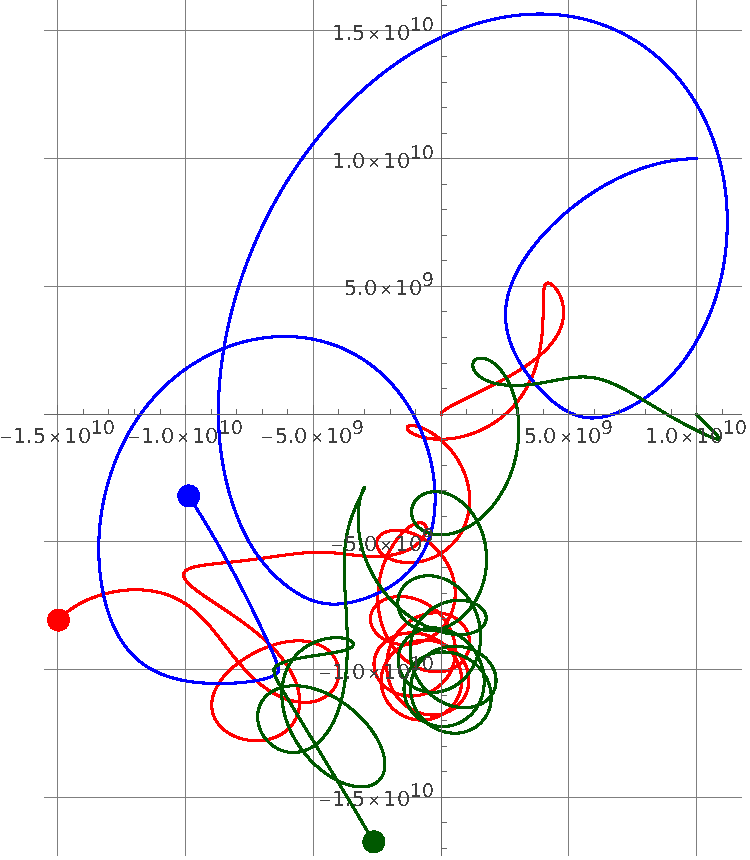
\includegraphics[width=0.7\linewidth]{img/simulation1.pdf}
}
\captionof{figure}{Stan symulacji I po $t = 9.5 \cdot 10^5~\mathrm{s}$.}
\end{minipage}

\subsubsection{Symulacja II}
\label{symulacja:ii}
\noindent
\begin{minipage}{\linewidth}
\captionsetup{type=figure}
Dane początkowe drugiej symulacji:

\begin{enumerate}
    \item \textbf{\textcolor{red}{Ciało Czerwone}}:
    \begin{itemize}
        \item $\vec{r}_0 = (0, 0)$
        \item $\vec{v}_0 = (5 \cdot 10^4, 10^4)~[\mathrm{\frac{m}{s}}]$
    \end{itemize}
    \item \textbf{\textcolor{blue}{Ciało Niebieskie}}:
    \begin{itemize}
        \item $\vec{r}_0 = (10^{10}, 0)~[\mathrm{m}]$
        \item $\vec{v}_0 = (-4 \cdot 10^4, 0)~[\mathrm{\frac{m}{s}}]$
    \end{itemize}
    \item \textbf{\textcolor{DarkGreen}{Ciało Zielone}}:
    \begin{itemize}
        \item $\vec{r}_0 = (5 \cdot 10^9, 7 \cdot 10^9)~[\mathrm{m}]$
        \item $\vec{v}_0 = (-8 \cdot 10^4, -2.5 \cdot 10^4)~[\mathrm{\frac{m}{s}}]$
    \end{itemize}
\end{enumerate}

Krok czasowy: $\dd t = 250~\mathrm{s}$
\vspace{2em}

\centering
\fbox{
    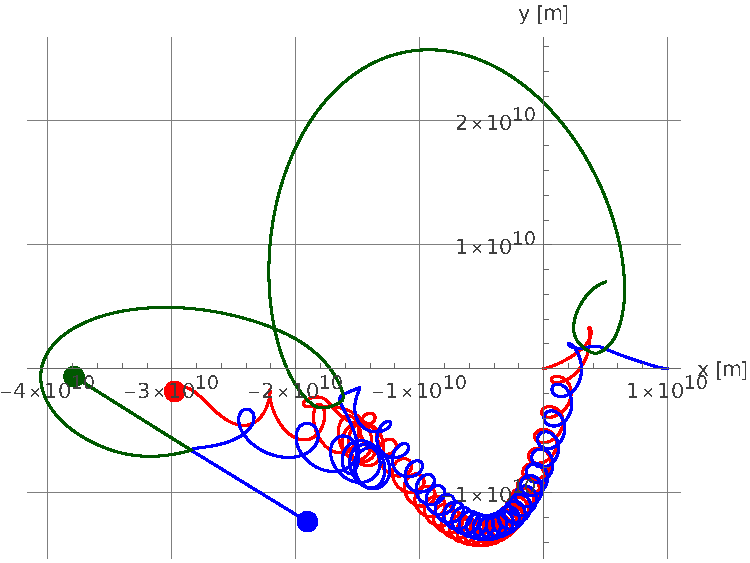
\includegraphics[width=0.9\linewidth]{img/simulation2.pdf}
}
\captionof{figure}{Stan symulacji II po $t \approx 1.45 \cdot 10^6~\mathrm{s}$.}
\end{minipage}

\subsection{Jedno ciało znacznie cięższe od pozostałych}
\subsubsection{Symulacja III}
\label{symulacja:iii}
\noindent
\begin{minipage}{\linewidth}
\captionsetup{type=figure}
Dane początkowe symulacji:

\begin{enumerate}
    \item \textbf{\textcolor{red}{Ciało Czerwone}}:
    \begin{itemize}
        \item $M = M_{\astrosun}$
        \item $\vec{r}_0 = (0, 0)$
        \item $\vec{v}_0 = (0, 0)$
    \end{itemize}
    \item \textbf{\textcolor{blue}{Ciało Niebieskie}}:
    \begin{itemize}
        \item $M = 10^{-4} M_{\astrosun}$
        \item $\vec{r}_0 = (0, 2 \cdot 10^9)~[\mathrm{m}]$
        \item $\vec{v}_0 = (3 \cdot 10^5, 0)~[\mathrm{\frac{m}{s}}]$
    \end{itemize}
    \item \textbf{\textcolor{DarkGreen}{Ciało Zielone}}:
    \begin{itemize}
        \item $M = 10^{-4} M_{\astrosun}$
        \item $\vec{r}_0 = (0, -5 \cdot 10^9)~[\mathrm{m}]$
        \item $\vec{v}_0 = (-2 \cdot 10^5, 0)~[\mathrm{\frac{m}{s}}]$
    \end{itemize}
\end{enumerate}

Krok czasowy: $\dd t = 2~000~\mathrm{s}$
\vspace{2em}

\centering
\fbox{
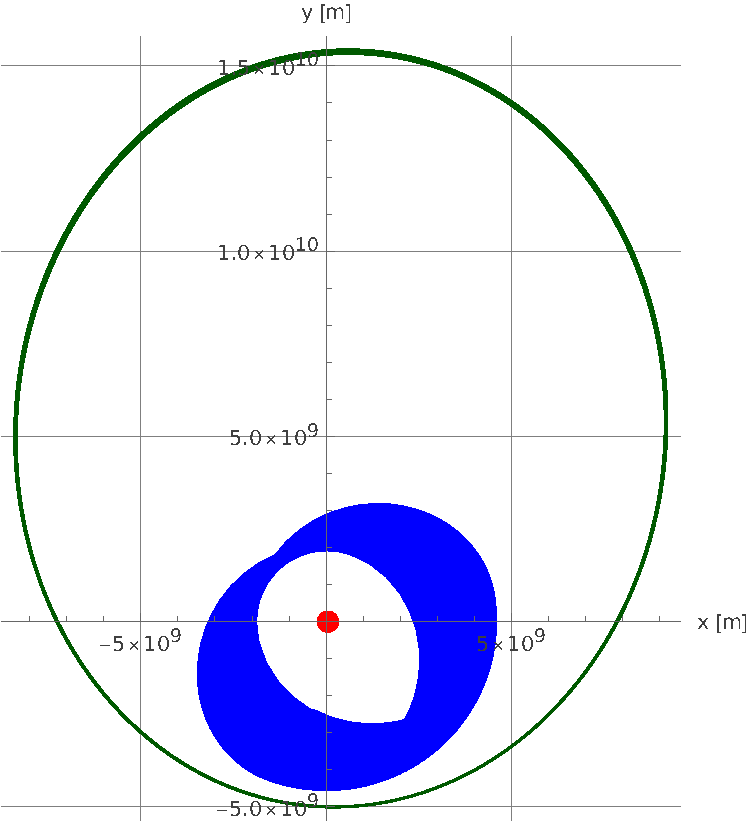
\includegraphics[width=0.75\linewidth]{img/simulation3.pdf}
}
\captionof{figure}{Stan symulacji III po $t = 5 \cdot 10^6~\mathrm{s}$.}
\end{minipage}

\subsection{Jedno ciało znacznie lżejsze od dwóch pozostałych}

\subsubsection{Symulacja IV}
\label{symulacja:iv}
\noindent
\begin{minipage}{\linewidth}
\captionsetup{type=figure}
Dane początkowe symulacji:

\begin{enumerate}
    \item \textbf{\textcolor{red}{Ciało Czerwone}}:
    \begin{itemize}
        \item $M = M_{\astrosun}$
        \item $\vec{r}_0 = (0, 0)$
        \item $\vec{v}_0 = (5 \cdot 10^4, 0)~[\mathrm{\frac{m}{s}}]$
    \end{itemize}
    \item \textbf{\textcolor{blue}{Ciało Niebieskie}}:
    \begin{itemize}
        \item $M = M_{\astrosun}$
        \item $\vec{r}_0 = (0, 10^{10})~[\mathrm{m}]$
        \item $\vec{v}_0 = (-5 \cdot 10^4, 0)~[\mathrm{\frac{m}{s}}]$
    \end{itemize}
    \item \textbf{\textcolor{DarkGreen}{Ciało Zielone}}:
    \begin{itemize}
        \item $M = 10^{-4} M_{\astrosun}$
        \item $\vec{r}_0 = (5 \cdot 10^8, 10^{10})~[\mathrm{m}]$
        \item $\vec{v}_0 = (-5 \cdot 10^4, -5 \cdot 10^5)~[\mathrm{\frac{m}{s}}]$
    \end{itemize}
\end{enumerate}

Krok czasowy: $\dd t = 2~500~\mathrm{s}$
\vspace{2em}

\centering
\fbox{
    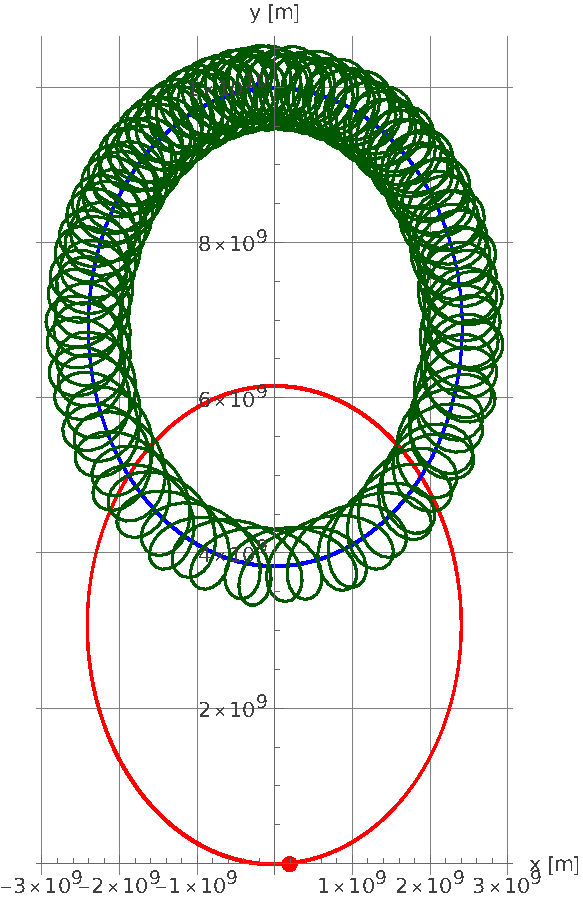
\includegraphics[width=0.55\linewidth]{img/simulation4.pdf}
}
\captionof{figure}{Stan symulacji IV po $t = 7.5 \cdot 10^5~\mathrm{s}$.}
\end{minipage}

\subsubsection{Symulacja V}
\label{symulacja:v}
\noindent
\begin{minipage}{\linewidth}
\captionsetup{type=figure}
Dane początkowe symulacji:

\begin{enumerate}
    \item \textbf{\textcolor{red}{Ciało Czerwone}}:
    \begin{itemize}
        \item $M = M_{\astrosun}$
        \item $\vec{r}_0 = (0, 0)$
        \item $\vec{v}_0 = (5 \cdot 10^4, 0)~[\mathrm{\frac{m}{s}}]$
    \end{itemize}
    \item \textbf{\textcolor{blue}{Ciało Niebieskie}}:
    \begin{itemize}
        \item $M = M_{\astrosun}$
        \item $\vec{r}_0 = (0, 10^{10})~[\mathrm{m}]$
        \item $\vec{v}_0 = (-5 \cdot 10^4, 0)~[\mathrm{\frac{m}{s}}]$
    \end{itemize}
    \item \textbf{\textcolor{DarkGreen}{Ciało Zielone}}:
    \begin{itemize}
        \item $M = 10^{-4} M_{\astrosun}$
        \item $\vec{r}_0 = (2 \cdot 10^9, 10^{10})~[\mathrm{m}]$
        \item $\vec{v}_0 = (-8 \cdot 10^3, -2.5 \cdot 10^5)~[\mathrm{\frac{m}{s}}]$
    \end{itemize}
\end{enumerate}

Krok czasowy: $\dd t = 50~\mathrm{s}$
\vspace{2em}

\centering
\fbox{
    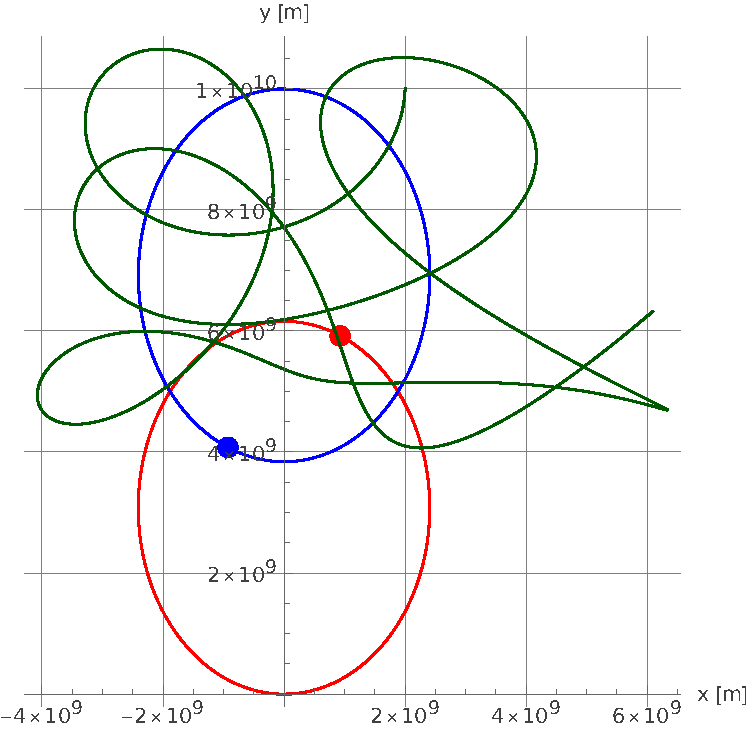
\includegraphics[width=0.8\linewidth]{img/simulation5.pdf}
}
\captionof{figure}{Stan symulacji V po $t \approx 3.27 \cdot 10^5~\mathrm{s}$.}
\end{minipage}

\subsubsection{Symulacja VI}
\label{symulacja:vi}
\noindent
\begin{minipage}{\linewidth}
\captionsetup{type=figure}
Dane początkowe symulacji:

\begin{enumerate}
    \item \textbf{\textcolor{red}{Ciało Czerwone}}:
    \begin{itemize}
        \item $M = M_{\astrosun}$
        \item $\vec{r}_0 = (0, 0)$
        \item $\vec{v}_0 = (6 \cdot 10^3, 0)~[\mathrm{\frac{m}{s}}]$
    \end{itemize}
    \item \textbf{\textcolor{blue}{Ciało Niebieskie}}:
    \begin{itemize}
        \item $M = \frac{1}{10} M_{\astrosun}$
        \item $\vec{r}_0 = (0, 10^{10})~[\mathrm{m}]$
        \item $\vec{v}_0 = (-6 \cdot 10^4, 0)~[\mathrm{\frac{m}{s}}]$
    \end{itemize}
    \item \textbf{\textcolor{DarkGreen}{Ciało Zielone}}:
    \begin{itemize}
        \item $M = 10^{-4} M_{\astrosun}$
        \item $\vec{r}_0 = (4 \cdot 10^8, 10^{10})~[\mathrm{m}]$
        \item $\vec{v}_0 = (-6 \cdot 10^4, 1.5 \cdot 10^5)~[\mathrm{\frac{m}{s}}]$
    \end{itemize}
\end{enumerate}

Krok czasowy: $\dd t = 250~\mathrm{s}$
\vspace{2em}

\centering
\fbox{
    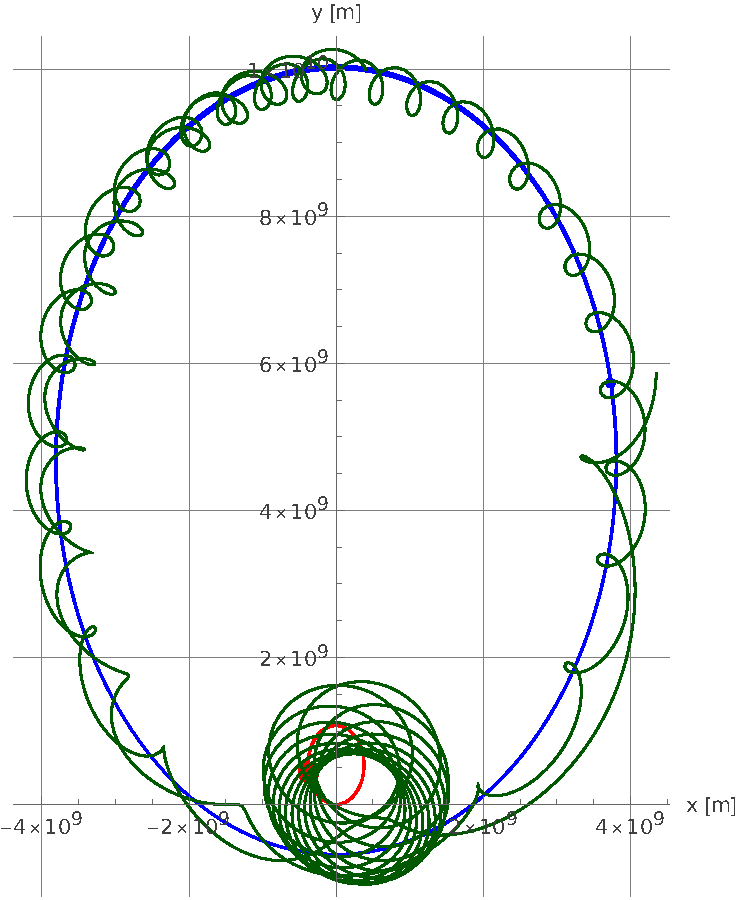
\includegraphics[width=0.75\linewidth]{img/simulation6.pdf}
}
\captionof{figure}{Stan symulacji VI po $t \approx 6.28 \cdot 10^5~\mathrm{s}$.}
\end{minipage}

\section{Dyskusja}
Podczas przygotowywania symulacji łatwo się przekonać jak bardzo chaotyczny jest to układ. Nawet zaniedbywalna zmiana parametrów początkowych zupełnie zmienia efekt końcowy. Dodatkowo widać jak na dłoni, że rozwiązanie numeryczne jest jedynie przybliżeniem rzeczywistości. Zmiana kroku czasowego również często prowadzi do zupełnie innego efektu końcowego symulacji.\br

Dla wariantu trzech ciał o identycznych masach niezwykle ciężko było mi znaleźć parametry, które nie doprowadziłyby do bardzo szybkiego \enquote{wystrzelenia} jednego z ciał poza strefę oddziaływania grawitacyjnego pozostałych. Obserwacje mówiące o tym, że w znaczącej większości układów do takiego \enquote{wystrzelenia} prędzej lub później dojdzie, można znaleźć w literaturze naukowej.\br

\textbf{Symulacja I} (\ref{symulacja:i}) oraz \textbf{Symulacja II} (\ref{symulacja:ii}) także kończy się \enquote{wystrzeleniem} ciał poza układ, jednak może to być kwestia zbyt małego kroku czasowego. Możliwe również, że w rzeczywistości doszłoby do zderzenia dwóch ciał, czego symulacja nie przewiduje.\br

\textbf{Symulacja III} (\ref{symulacja:iii}) jest już układem znacznie bardziej stabilnym. Zgodnie z przewidywaniem, wpływ lekkich ciał na siebie nawzajem jest znikomy i powstały układ przypomina zachowanie układu planetarnego. Drobne zmiany parametrów początkowych nie prowadzą do drastycznych zmian efektu końcowego. Zmiana kroku czasowego wpływa jednak na charakter \enquote{precesji} ciała niebieskiego.\br

\textbf{Symulacja IV} (\ref{symulacja:iv}) także ma dość stabilny charakter. Ciało zielone jest zdominowane grawitacyjnie przez ciało niebieskie, przez co trzecie z ciał nie ma wyraźnego wpływu na ruch lekkiego ciała. Sytuacja ta przypomina nieco układ Gwiazda-Planeta-Księżyc.\br

W wyniku zwiększenie orbity zielonego satelity z \textbf{Symulacji IV} (\ref{symulacja:iv}) otrzymujemy \textbf{Symulację V} (\ref{symulacja:v}). Z racji na fakt, że nie ma już tak wyraźnej różnicy w odległościach ciała lekkiego, od pozostałych ciał ciężkich, ciało lekkie zostaje dość szybko \enquote{wystrzelone} z układu.\br

Bardzo ciekawa sytuacja ma miejsce w \textbf{Symulacji VI} (\ref{symulacja:vi}). Ciało zielone, będące na początku satelitą ciała niebieskiego, zostaje \enquote{przejęte} przez najcięższe ciało czerwone. Sytuacja ta zmienia się jednak po pewnym czasie ponownie, gdy ciało niebieskie przelatuje na tyle blisko zielonego, że jest w stanie z powrotem \enquote{wydrzeć grawitacyjnie} swojego satelitę.\br

\section{Literatura}
\bibliographystyle{alpha}
\bibliography{references}

\end{document}
